\begin{frame}{Numerical Method implemented}
The numerical method currently implemented are:
  \begin{itemize}
    \item Variational Multiscale Method (VMS)
    \item Streamline upwind Petrov–Galerkin (SUPG)
  \end{itemize} 

Different solution method are available for all of them 
  \begin{itemize}
    \item Non-linear (NLIN)
    \item Linearized-Coupled (LC-VMS)
    \item Linearized-Segregated (LS-VMS)
  \end{itemize} 
\end{frame}


\begin{frame}{Variational Multiscale Method}
  \begin{itemize}
    \item Evolution of the SUPG
    \item Implict LES
    \item It does not need calibration
    \item Residual-based stabilization
  \end{itemize} 
\end{frame}


\begin{frame}{Galkerkin formulation}
Conservation of mass:
\begin{equation}
    \nabla\cdot \Vec{u} = 0
    \label{equfo:cont}
\end{equation}

Conservation of momentum:
\begin{equation}
    \dfrac{\partial \Vec{u}}{\partial t} + (\Vec{u}\cdot\nabla)\Vec{u} + \nabla p - \nu\Delta\Vec{u} - f = 0
        \label{equfo:mom}
\end{equation}

Variational Formulation
\begin{equation}
\begin{split}
  B^G = &   \int_\Omega \dfrac{\partial \Vec{u}}{\partial t}\cdot \Vec{v}\;d\Omega +
    \int_\Omega(\Vec{u}\cdot\nabla)\Vec{u}\cdot \Vec{v} \;d\Omega+ 
    \int_\Omega \nabla (p)\cdot\Vec{v} \;d\Omega + \\
     & \int_\Omega\nu\nabla\Vec{u}\cdot\nabla\Vec{v} \;d\Omega  -
        \int_\Omega f\cdot\Vec{v} \;d\Omega + 
    \int_\Omega q(\nabla \cdot \Vec{u})\;d\Omega = 0
    \end{split}
    \label{equ:weak}
\end{equation}

\end{frame}

\begin{frame}{Stabilization equations}
\begin{equation}
B^{SUPG}(t, (\Vec{u},p), (\Vec{v},q))  =     \int_\Omega(\tau_m(\Vec{u}\cdot\nabla \Vec{v} +\nabla q)\cdot\Vec{R_m} \;d\Omega+ \int_\Omega \tau_c (\nabla \cdot \Vec{v})R_c \;d\Omega
\label{equ:bsupg}
\end{equation}

\begin{equation}
B^{VMS1}(t, (\Vec{u},p), (\Vec{v},q))  = \int_\Omega (\Vec{u}\cdot\nabla \Vec{v}')\odot(\tau_m \Vec{R_m}) \;d\Omega
\label{equ:bvms1}
\end{equation}


\begin{equation}
B^{VMS2}(t, (\Vec{u},p), (\Vec{v},q))  = -\int_\Omega (\nabla\Vec{v}\odot(\tau_m \Vec{R_m} \otimes \tau_m \Vec{R_m}) \;d\Omega
\label{equ:bvms2}
\end{equation}

\end{frame}


\begin{frame}{Stabilization parameters}

\begin{equation}
\tau_m =\bigg( \dfrac{4}{\Delta t^2} + \Vec{u}\cdot{G}\Vec{u} + C_I \nu^2 {G}:{G} \bigg)^{-1/2}
\label{equ:taum}
\end{equation}

\begin{equation}
\tau_c = (\tau_c\Vec{g}\cdot\Vec{g})^{-1}
\label{equ:tauc}
\end{equation}

Where G is the inverse of the gradient of the map cell.
For a cubed shaped element, with $h$ the edge length, $G_{ij} =\dfrac{1}{h^2}\delta_{ij}$, where $\delta_{ij}$ is the Kronecker delta.

\end{frame}


\begin{frame}{Linearization}

\begin{equation}
    \tilde{\Vec{u}} = 2.1875 u^{n} - 2.1875 u^{n-1} + 1.3125 u^{n-2} - 0.3125 u^{n-3} 
    \label{equlin:taylor_exp}
\end{equation}

\begin{equation}
 (\Vec{u}\cdot\nabla)\Vec{u} \Rightarrow  (\tilde{\Vec{u}} \cdot\nabla)\Vec{u} 
\end{equation}


\end{frame}



\begin{frame}{Boundary Layer Initialization}
\begin{itemize}
\item Avoid Instabilities (close to the leading edge)
\item Avoid velocity ramping
\item Higher time-step
\end{itemize}
Using the function exploited by RANS solvers for the wall distance for computing turbulent parameters but now used to detect the airfoil's contour
\begin{equation}
\begin{cases}
    \nabla \cdot (|\nabla u_p|^{p-2} \nabla u_p) = -1 & x\in \Omega\\
    u_p = 0 & x\in \Omega_D
    \end{cases}
    \label{equ:ppoisson}
\end{equation}
The true-wall distance is provided by solving the equation for $p\xrightarrow{}\infty$
Solved using a method that resembles Picard's
\end{frame}

\begin{frame}{Boundary Layer Initialization}
The velocity in the $x$ direction in the region identified can be with a simple cubic function \eqref{equ:bl-cubic-init} where $dn = d/\delta_{99}$, $d$ is the minimum distance to the airfoil, $u_\infty$ is the free-stream flow speed.
\begin{equation}
    f(dn) = 
    \begin{cases}
        u_\infty & dn>1\\
        ( -dn^2+2\cdot dn )\cdot u_\infty &  dn<1
    \end{cases}
    \label{equ:bl-cubic-init}
\end{equation}
 The boundary layer function has been obtained by fixing the following boundary conditions:
\begin{itemize}
    \item Continuity with the external flow, $f(1)=1$ 
    \item Smooth transition between boundary layer and external flow, $f'(1)=0$ 
    \item Non-slip condition at the wall, $f(0)=0$
\end{itemize}
\end{frame}

\begin{frame}{Boundary Layer Initialization}
It results in a low-speed zone close to the airfoil, avoiding high speed in really small cells useful for capturing the boundary layer.
\begin{figure}
         \centering
         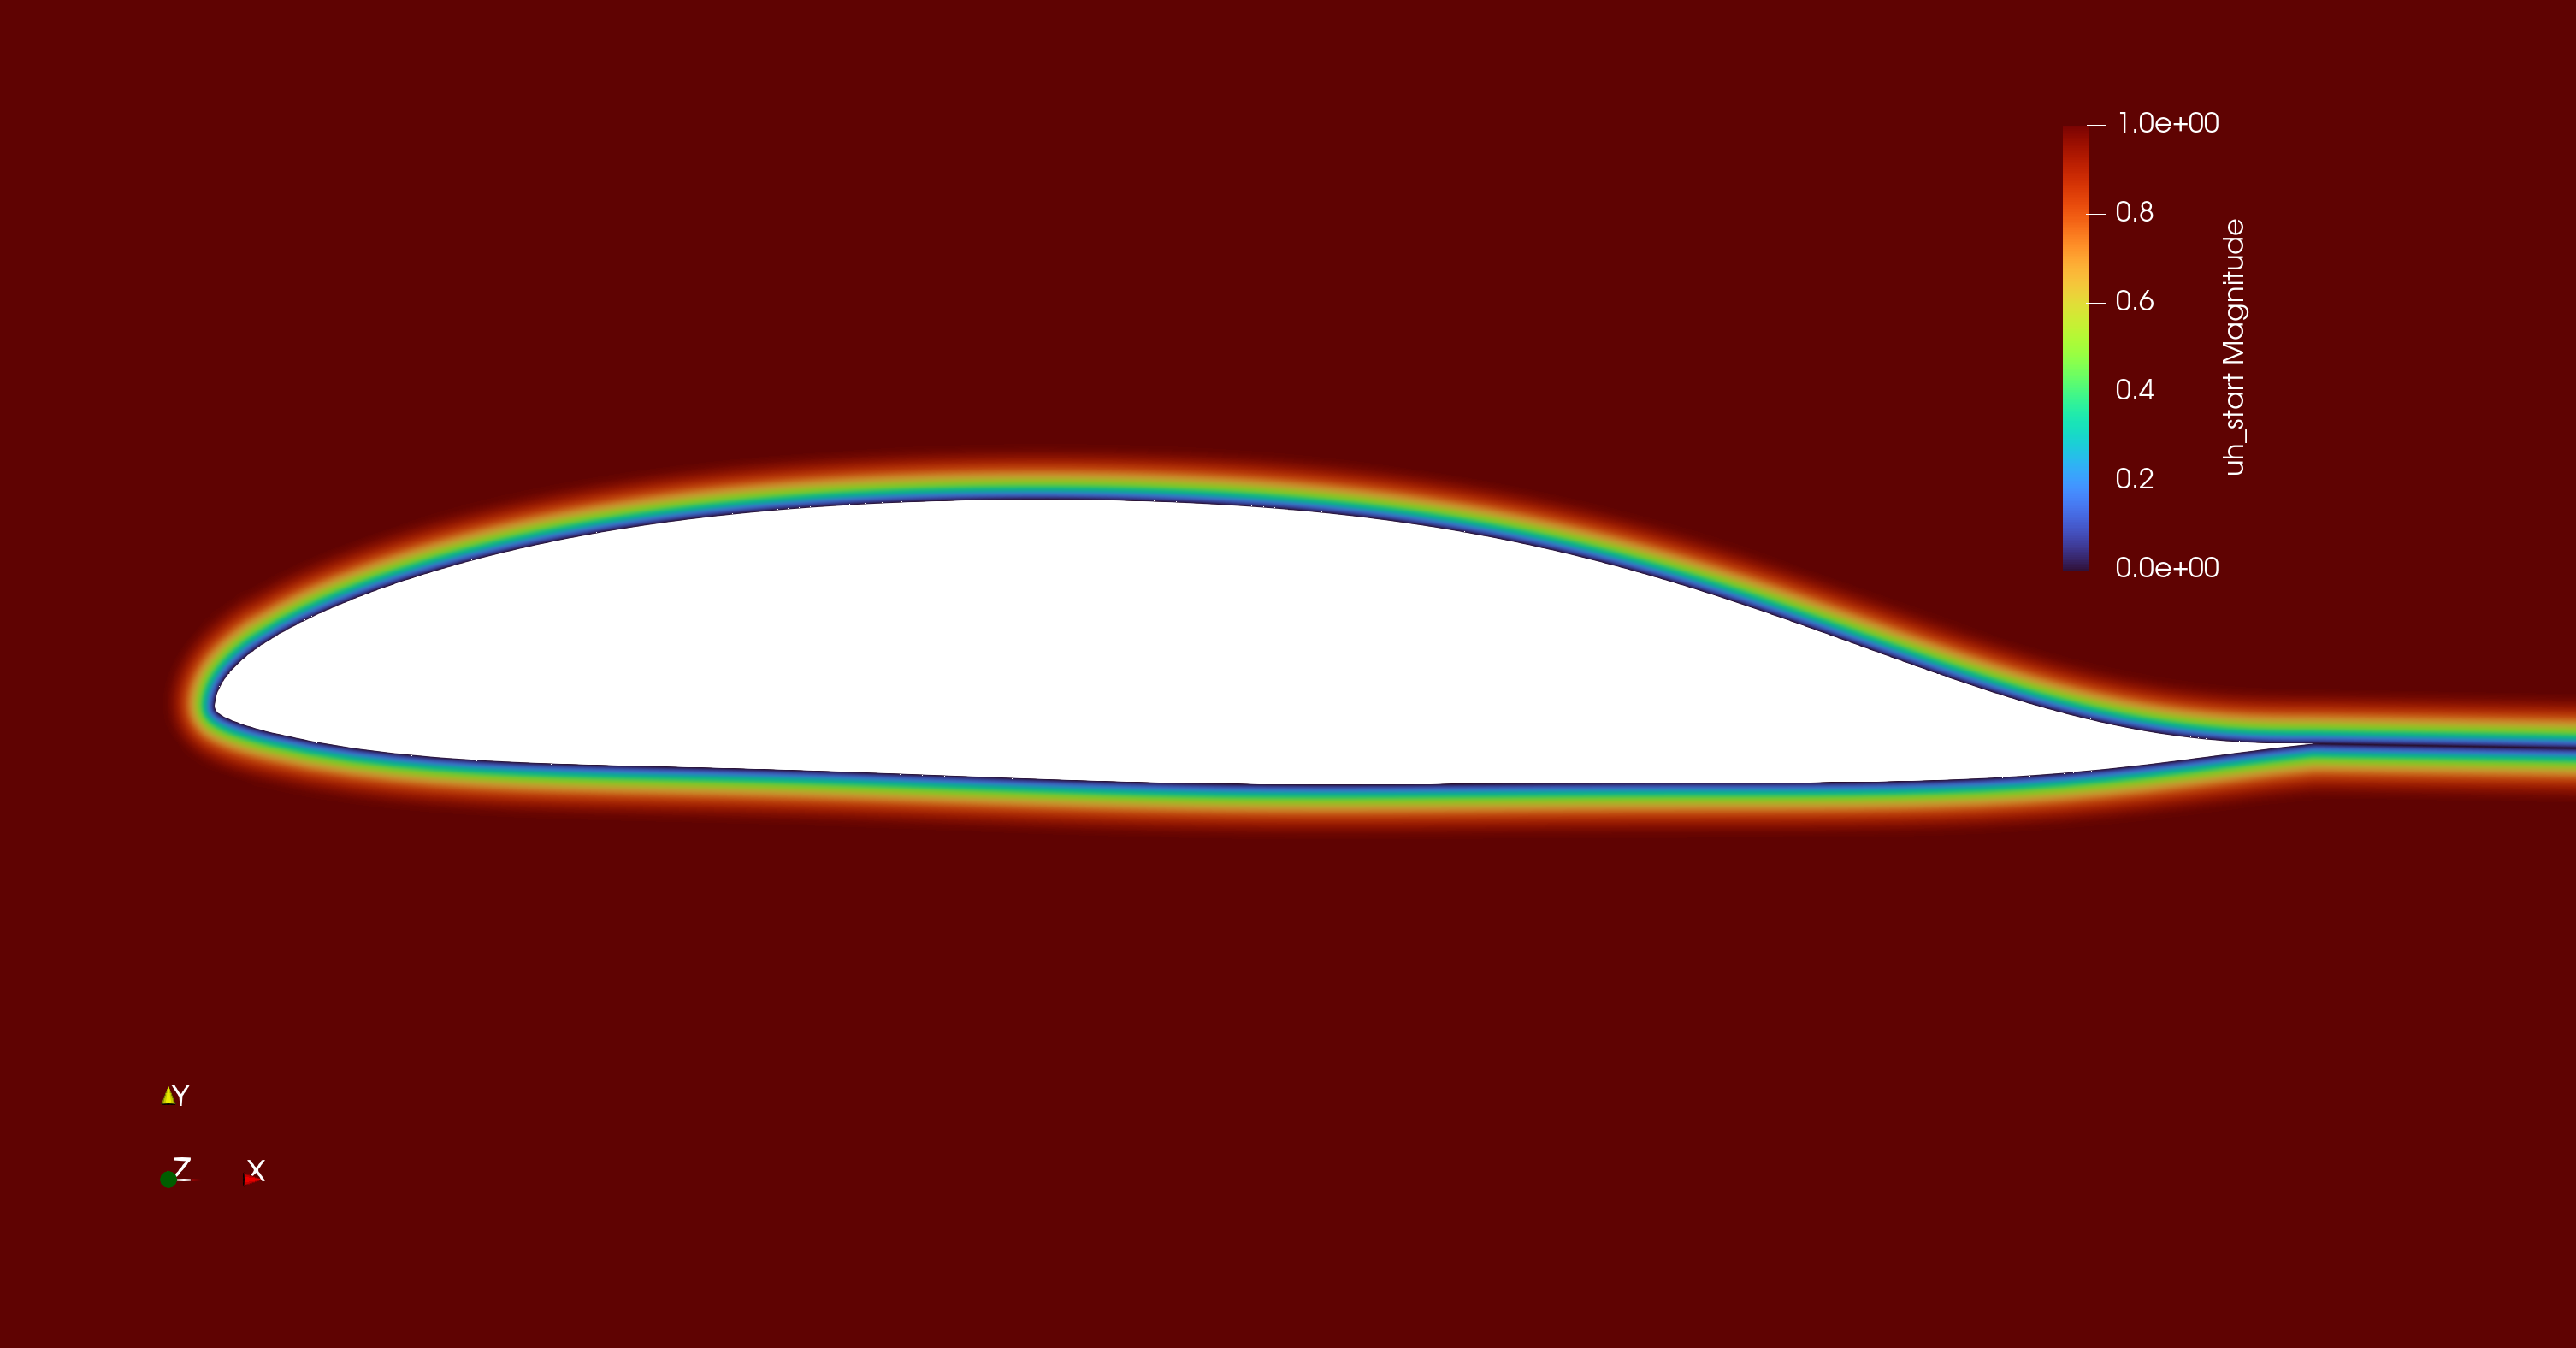
\includegraphics[width=0.65\textwidth]{WallDistanceDU89.png}
         \caption{Boundary Layer Initialization}
         \label{fig:wall-distance-init}
\end{figure} 
\end{frame}
